In diesem Abschnitt werden die bekannten Funktionsweisen und Nachrichten von FastTrack beschrieben.
Dabei werden die Informationen in allen folgenden Abschnitten aus der Studie \cite{liang2006fasttrack} von genommen.
Zuerst werden in \ref{subsec:nachricht} auf die Nachrichten, welche über FastTrack verschickt werden, beschrieben.
Danach wird im Abschnitt \ref{subsec:join} das Verbinden zum FastTrack Netzwerk dargestellt.
Es wird dann in \ref{subsec:sntosn} der Austausch von Metadaten zwischen Superknoten beschrieben.
Im Anschluss wird in \ref{subsec:search} auf die Suche im Netzwerk eingegangen.

\subsection{Nachrichten}
\label{subsec:nachricht}

Im FastTrack Netzwerk gibt es vier verschiedene Nachrichtentypen für den Austausch von Informationen. Folgende Nachrichtentypen gibt es:

\begin{itemize}
\item[1.] \textbf{Signal Nachrichten:} Diese Nachrichten dienen zum Austausch von Informationen im Netzwerk.
Zum einen um mitzuteilen, wenn sich ein Knoten das Netzwerk betreten will.
Ein Knoten Metainfomationen zum SN senden will oder ein SN aktuelle Informationen seines SN Caches mit einen normalen Knoten oder anderen SN austauschen will.
Außerdem werden darüber die Suchanfragen geschickt.
Wichtig ist, dass alle Signal Nachrichten verschlüsselt übertragen werden.
Deshalb muss am Anfang einer Übertragung ein Schlüssel ausgetauscht werden.
\item[2.] \textbf{Daten Transport Nachrichten:} Dieser Nachrichtentyp wird zum Austausch von Daten verwendet. 
Dabei werden diese Nachrichten nicht verschlüsselt übertragen.
Für die Übertragung der Rohdaten wird HTTP verwendet.
\item[3.] \textbf{Advertise Nachrichten:} Da hinter FastTrack Firmen stehen die mittels der Werbung Geld verdient, gibt es ein Nachrichtentyp um die Werbung zu übertragen.
Dies geschieht unverschlüsselt über HTTP Nachrichten.
\item[4.] \textbf{Sofort Nachrichten:} Damit es eine Möglichkeit gibt, dass sich zwei Teilnehmer des Netzwerkes unterhalten können, gibt es Sofort Nachrichten.
In diesen werden nur Text Nachrichten übertragen.
Damit die Unterhalten nicht mit gelesen werden kann, werden diese verschlüsselt übertragen.
\end{itemize} 

\subsubsection{Signal Nachrichten}
\label{subsubsec:sigN}

In der Abbildung \ref{fig:sigN} ist der Aufbau der Signalnachrichten dargestellt.
Die \textit{Packet ID} enthält die ID des Paketes um die Nachricht zu identifizieren.
Dafür wird 1 Byte verwendet.
Im \textit{Message Type} wird angegeben, ob eine Verbindung aufgebaut werden soll, Metadaten versendet oder SN-Listen ausgetauscht werden.
Es werden dafür 2 Byte verwendet.
Der \textit{Payload} enthält die Metadaten oder SN-Listen.
Die Länge des \textit{Payload} wird in der \textit{Payload Length} gespeichert
Dafür stehen in der Nachricht 2 Byte zur Verfügung.

\begin{figure}
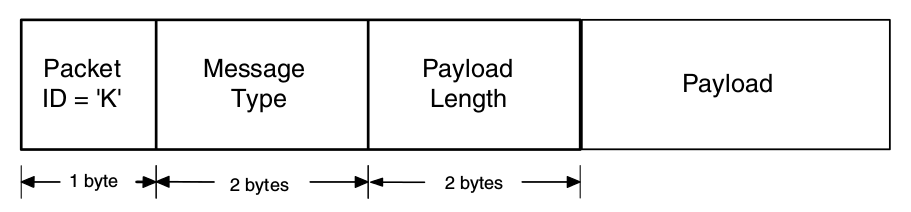
\includegraphics[scale=0.25]{gfx/signal_message}
\caption{Signal Nachricht (Quelle \cite{liang2006fasttrack})}
\label{fig:sigN}
\end{figure}

\subsection{Dem Netzwerk beitreten}
\label{subsec:join}

Der Ablauf, wenn sich ein Knoten in FastTrack Netzwerk verbindet ist in Abbildung \ref{fig:join} dargestellt.
Zuerst wählt der Knoten aus dem eigenen SN Cache ein paar SN.
Zu den gewählten SN wird eine \textit{UPD probe} Nachricht geschickt um zu testen ob der SN antworten.
Nachdem der SN geantwortet hat, wird ein TCP Handshake durchgeführt. 
Danach findet der Schlüsselaustausch statt, damit die folgenden Nachrichten verschlüsselt werden können.
Nun sendet der Knoten die Metadaten seiner Dateien zum SN.
Darunter ist auch die lokale IP, der Port und der Benutzername, des Knoten.
Mit der lokalen IP wird verhindert, dass nur der SN weiß, wo die Daten zu finden sind.
Der SN wiederum sendet eine Liste seiner bekannten SNs zum Knoten zurück.
Mit dieser Liste aktualisiert der Knoten seinen SN Cache.
Wenn der SN Cache aktualisiert ist, bricht der Knoten die Verbindung ab und sucht sich aus der aktualisierte Listen einen Eltern SN. 
Mit welchem er sich verbindet und ihm seine Metadaten und lokale Information schickt.
Die Möglichkeit der Wahl des Eltern SN wird in \ref{subsubsec:wElternSN} erläutert.
An diesem Eltern SN kann nun die Suchanfragen geschickt werden.

\begin{figure}
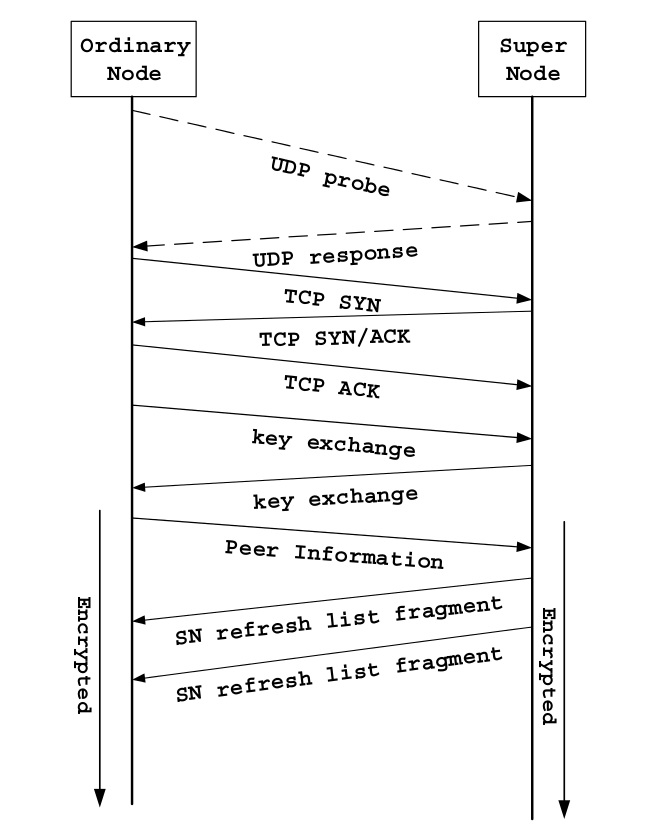
\includegraphics[scale=0.3]{gfx/join}
\caption{Nachrichten beim Verbindungsaufbau (Quelle \cite{liang2006fasttrack})}
\label{fig:join}
\end{figure}

\subsubsection{Wahl des Eltern SN}
\label{subsubsec:wElternSN}

Im Paper \cite{liang2006fasttrack} ist beschrieben, das nicht genau bekannt ist, nach welchen Kriterien der Eltern SN gewählt wird. 
Es werden zwei Möglichkeiten in Betracht gezogen.
Zum einen die Lokalität, dass heißt wie weit der SN vom Knoten entfernt ist und zum anderen die Auslastung des SN.
Bei der Lokalität wird der RoundTripTime durch einen Ping zum SN gemessen.
In der Messung \ref{fig:rtt} ist zu erkennen, dass die meisten Knoten mit SN in ihrer Nähe verbunden sind.
Ein anderer Aspekt ist die Auslastung eines SN.
Dabei spielt es eine Rolle wie viele normale Knoten ein SN schon verwaltet.
Die Information der Auslastung wird mit im SN Cache des Knoten gespeichert, welcher beim betreten des Netzwerkes aktualisiert ist.
In der Abbildung \ref{fig:workl} ist zu erkennen, dass in der Messung der Eltern SN durchschnittlich mit einer geringen Auslastung gewählt werden.
Somit sind beide Kriterien, die Lokalität sowie die Auslastung des SN, ausschlaggebend in der Wahl des Eltern SN.

\begin{figure}
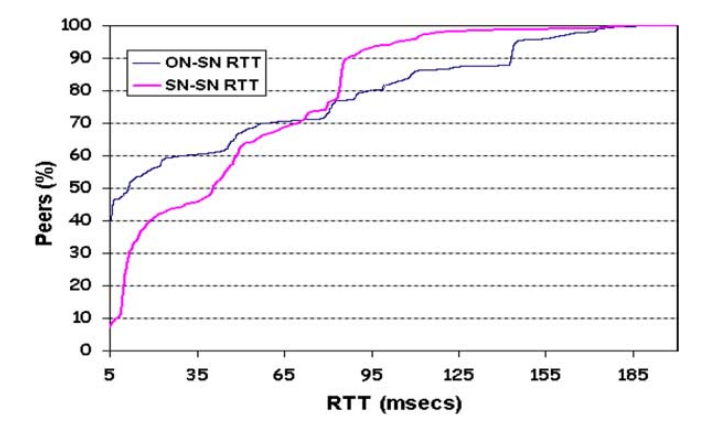
\includegraphics[scale=0.3]{gfx/rttSns}
\caption{RTT Knoten zu SN und SN zu SN (Quelle \cite{liang2006fasttrack})}
\label{fig:rtt}
\end{figure}

\begin{figure}
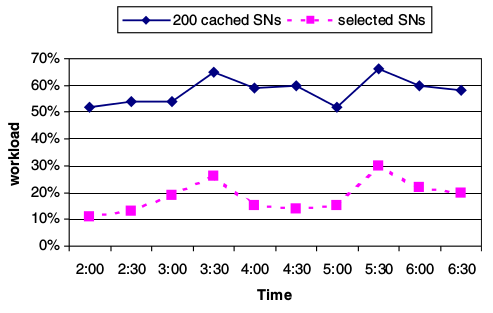
\includegraphics[scale=0.45]{gfx/workload}
\caption{Auswahl des Eltern SN nach Auslastung (Quelle \cite{liang2006fasttrack})}
\label{fig:workl}
\end{figure}

\subsection{Datenaustausch zwischen Superknoten}
\label{subsec:sntosn}

Der Ablauf wie die Superknoten untereinander ihre Daten austauschen ist in der Abbildung \ref{fig:snsn} dargestellt.
Zuerst wählt der SN einen SN aus seinem Cache.
Mit dem gewählten SN wird ein TCP Handshake durchgeführt um sich zu verbinden.
Da die Nachrichten verschlüsselt werden sollen, wird nach dem TCP Handshake ein Schlüssel ausgetauscht.
Danach senden die SN verschlüsselt ihre aktuellen bekannten SNs um ihren Cache zu aktualisieren.

\begin{figure}
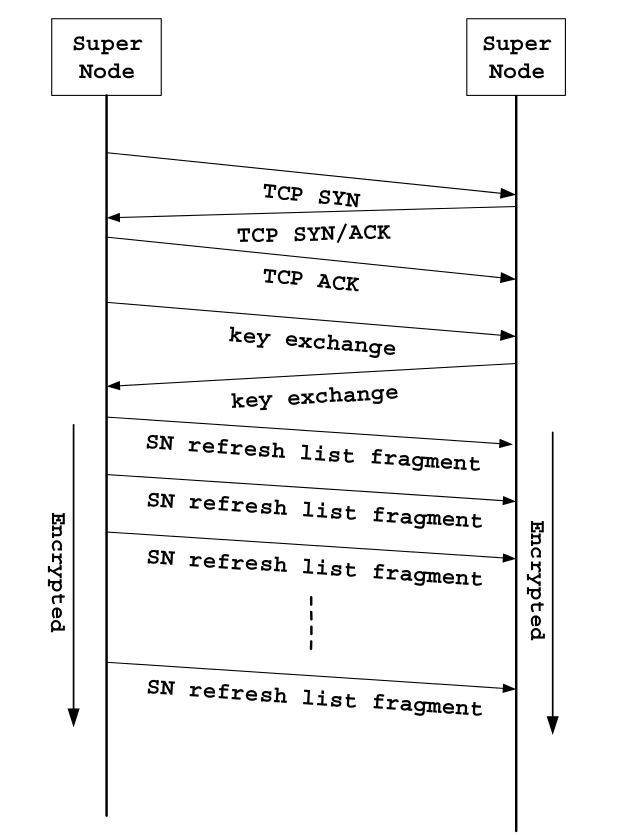
\includegraphics[scale=0.3]{gfx/SnToSn}
\caption{Nachrichten beim Austausch von Informationen zwischen SNs(Quelle \cite{liang2006fasttrack})}
\label{fig:snsn}
\end{figure}

\subsection{Suche im Netzwerk}
\label{subsec:search}

Wenn ein Knoten ein Datei suchen will, sendet dieser seinen Suchanfrage an seinen Eltern SN.
Dieser durchsucht die Metadaten seine bekannten Knoten anhand der Wörter in der Suchanfrage und schickt die Antwort ob etwas gefunden wird zurück.
Außerdem wird die Suchanfrage an seine bekannte SN gesendet, damit dieser in den Metadaten seiner bekannten Knoten.
Mit der Antwort, kann der Knoten nun den Download starten.
In Sektion \ref{subsubsec:dnat} wird beschrieben wie der Download stattfindet, wenn der Knoten, welcher die Datei besitzt hinter eine Nat sitzt.

\subsubsection{Download über NAT}
\label{subsubsec:dnat}
Da es häufig vorkommt, dass die Knoten B hinter einem NAT sitzen, gibt es die Möglichkeit über den Eltern SN des jeweiligen Knoten, den Download zu starten.
Wenn ein Knoten A einen Download starten will, dann hat er die IP Adresse des Knoten B, daran erkennt er ob es eine lokale oder globale Adresse handelt.
Bei einer lokalen Adresse fragt er den Eltern SN des Knoten B, dass er von Knoten B eine Datei herunterladen will und nur die lokale Adresse kennt.
Der Eltern SN von B, teilt nun Knoten B mit, das Knoten A eine Datei von ihm herunterladen will.
Diese Nachricht enthält die globale Adresse von A.
Nun verbindet sich Knoten B mit Knoten A und Knoten A kann die Datei von B herunterladen.